\documentclass[11pt,letterpaper,boxed]{hmcpset}

% include this package to customize page layout of document (e.g. to adjust margins)
\usepackage[margin=0.9in]{geometry}
\usepackage{ulem}

% set numbering style for enumerated lists to be of form (a), (b), (c), etc.
\renewcommand{\labelenumi}{{\bf (\alph{enumi})}}

%% Extra packages
\usepackage{amsfonts, amsmath, amssymb, enumerate, esvect, fancyhdr, gensymb, graphicx, lastpage, mathtools, mathrsfs, parskip}
%%

% Bold font shortcut
\renewcommand{\v}[1]{\textbf{#1}}

% info for header block in upper right hand corner
\name{Ki Pheng (Kip) Lim}
\class{Section 7}
\assignment{Mailbox \# 521}
\duedate{April 9, 2019}

\begin{document}
\problemlist{MATH045 HW4}

%------------------------- Problem 1 -----------------------

\begin{problem}[1]
(5 points) What linear, second-order, constant-coefficient, unforced DE can have $y(x) = Ce^{-5x} + De^{2x}$ as its general solution? Also, determine the characteristic equation that is consistent with this general solution.
\end{problem}

%\begin{solution}
%\end{solution}

\pagebreak

%------------------------- Problem 2 -----------------------

\begin{problem}[2]
(5 points) Complete the following.

\begin{enumerate}
\item Find the solution to the IVP $\ddot y + 21\dot y + 20y = 0$ with $y_0 = 0$, $\ddot y_0 = 19$.
\item Your answer to (a) is the sum of two exponential terms. Suppose t > 0. As t increases, which term is negligible and which dominates? Graph your answer to (a) along with the dominant exponential term by itself on the same axes to verify your answer.
\end{enumerate}
\end{problem}

%\begin{solution}
%\end{solution}

\pagebreak

%------------------------- Problem 3 -----------------------

\begin{problem}[3]
(5 points) Find the general solution to the following ODEs.

\begin{enumerate}
\item $y'' + 6y' + 8y = 0$
\item $y'' + 6y' + 9y = 0$
\item $y'' + 9y = 0$
\item $y'' + 4y = y'$
\end{enumerate}
\end{problem}

%\begin{solution}
%\end{solution}

\pagebreak

%------------------------- Problem 4 -----------------------

\begin {problem} [4]
(5 points) Consider the IVP $y'' + y' + y = 0$ with $y(0) = 1$ and $y_0(0) = 0$.

\begin {enumerate}
\item Solve this problem using complex exponentials instead of sines and cosines. When you have solved for your unknown constants, express them in complex exponential form. (That is, instead of writing it as $a + bi$, write it as $\alpha$ $ei$ $\theta$ for some $\alpha$ and $\theta$.) Leave your answer in complex exponential form.
\item Now, manipulate your solution in the following way, so as to convert your complex exponential solution into sines and cosines again. You should get a real-value function in the end and have a trig function involving a phase shift. Refer to Problem 1 from Homework 2.
\centering
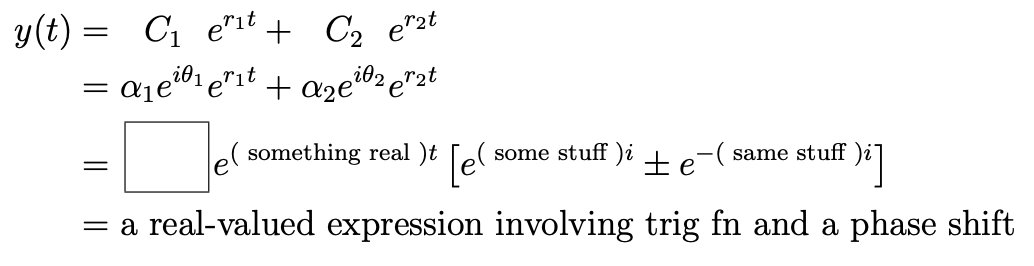
\includegraphics[width=100mm]{HW4/p4.png}
\end{enumerate}
Optional: Compare your solution with the solution that we obtained in class. Show that they are equivalent.
\end{problem}

%\begin{solution}
%\end{solution}

\pagebreak

%------------------------- Problem 5 -----------------------
\begin{problem}
(5 points) Consider the second-order, linear, constant-coefficient, unforced DE $ay'' + by' + cy = 0$. Suppose you know that the solutions to this differential equation decay to 0 as $t \rightarrow \infty$, regardless of what initial conditions are chosen. What must be true about the roots of the characteristic equation $a\lambda 2 + b\lambda + c = 0$? (This question does not require any calculations, but this idea is important enough that we are highlighting it in this problem.)
\end{problem}

%\begin{solution}
%\end{solution}

\pagebreak

\end{document}